
% License:
% CC BY-NC-SA 3.0 (http://creativecommons.org/licenses/by-nc-sa/3.0/)
%
%%%%%%%%%%%%%%%%%%%%%%%%%%%%%%%%%%%%%%%%%

%----------------------------------------------------------------------------------------
%	PACKAGES AND OTHER DOCUMENT CONFIGURATIONS
%----------------------------------------------------------------------------------------


\documentclass[paper=a4, fontsize=13pt, oneside, openany]{scrartcl} % A4 paper and 11pt font size
%%%%%%%%%%\clearpage & \cleardoublepa

\usepackage[T1]{fontenc} % Use 8-bit encoding that has 256 glyphs
\usepackage{fourier} % Use the Adobe Utopia font for the document - comment this line to return to the LaTeX default
\usepackage[english]{babel} % English language/hyphenation
\usepackage{amsmath,amsfonts,amsthm} % Math packages
\usepackage{lipsum} % Used for inserting dummy 'Lorem ipsum' text into the template
\usepackage{textcomp}
%\usepackage{xcolor,colortbl}


%\usepackage{natbib}%Harvard referencing package

\usepackage{caption}
\usepackage{subcaption}
\usepackage{graphicx}
\graphicspath{./images/}
\usepackage[dvipsnames]{xcolor,colortbl}
\usepackage{pdfpages}
\usepackage[title,toc,titletoc,page]{appendix}
\addappheadtotoc
\usepackage{dirtytalk} %for direct quotations



\usepackage{float}

\usepackage{blindtext} %for enumarations

\usepackage[]{hyperref}  %link collor
%\usepackage{hyperref}
\hypersetup{
    colorlinks=true,
    linkcolor= black,
    filecolor= Maroon,
    citecolor=black,
    urlcolor=MidnightBlue,
}


%talbe layout to the right
%\usepackage[labelfont=bf]{caption}
%\captionsetup[table]{labelsep=space,justification=raggedright,singlelinecheck=off}
%\captionsetup[figure]{labelsep=quad}

\usepackage{sectsty} % Allows customizing section commands
%\allsectionsfont{\centering \normalfont\scshape} % Make all sections centered, the default font and small caps
\allsectionsfont{ \normalfont\scshape} % Make all sections centered, the default font and small caps

\usepackage{fancyhdr} % Custom headers and footers
\pagestyle{fancyplain} % Makes all pages in the document conform to the custom headers and footers
\fancyhead{} % No page header - if you want one, create it in the same way as the footers below
\fancyfoot[L]{} % Empty left footer
\fancyfoot[C]{} % Empty center footer
\fancyfoot[R]{\thepage} % Page numbering for right footer
\renewcommand{\headrulewidth}{0pt} % Remove header underlines
\renewcommand{\footrulewidth}{0pt} % Remove footer underlines
\setlength{\headheight}{13.6pt} % Customize the height of the header

\numberwithin{equation}{section} % Number equations within sections (i.e. 1.1, 1.2, 2.1, 2.2 instead of 1, 2, 3, 4)
\numberwithin{figure}{section} % Number figures within sections (i.e. 1.1, 1.2, 2.1, 2.2 instead of 1, 2, 3, 4)
\numberwithin{table}{section} % Number tables within sections (i.e. 1.1, 1.2, 2.1, 2.2 instead of 1, 2, 3, 4)

%\setlength\parindent{0pt} % Removes all indentation from paragraphs - comment this line for an assignment with lots of text


\setlength\parskip{4pt}

%----------------------------------------------------------------------------------------
%	TITLE SECTION
%----------------------------------------------------------------------------------------
\begin{document}
\begin{titlepage}
\begin{center}
        \vspace*{3cm}

        \Huge
        \textit{PhD Transfer Report}\\[15pt]
 
        \vspace{0.5cm}
        \LARGE
        Student Name
 
        \vspace{0.2cm}
        \normalfont\Large
        March 2022
        
        \vspace{9.5cm}
 
        
\includegraphics[width=0.6\textwidth]{Images/city-logo.png}
 
 
    \end{center}
\end{titlepage}


\newpage
\tableofcontents

\newpage
\section{Introduction}

\lipsum[5]
Citing this author \cite{Fleetwood_2017}.
\lipsum[5]

\lipsum[5]

\subsection{Introduction topic}

\lipsum[5]

\lipsum[5]

\newpage
\section{Background/Related Work}

\lipsum[5]

\lipsum[5]

\lipsum[5]

\subsection{Related work topic}

\lipsum[5]

\lipsum[5]

\newpage
\section{Research Hypotheses/Questions}

\lipsum[5]

\lipsum[5]

\lipsum[5]

\subsection{Research questions topic}

\lipsum[5]

\lipsum[5]

\newpage
\section{Methods}

\lipsum[5]

\lipsum[5]

\lipsum[5]

\subsection{Methods topic}

\lipsum[5]

\lipsum[5]

\newpage

 \section{Research Plan}
 
\lipsum[5]

\lipsum[5]

\lipsum[5]

\subsection{Research plan topic}

\lipsum[5]

\lipsum[5]

\begin{figure}[h!]
\centering
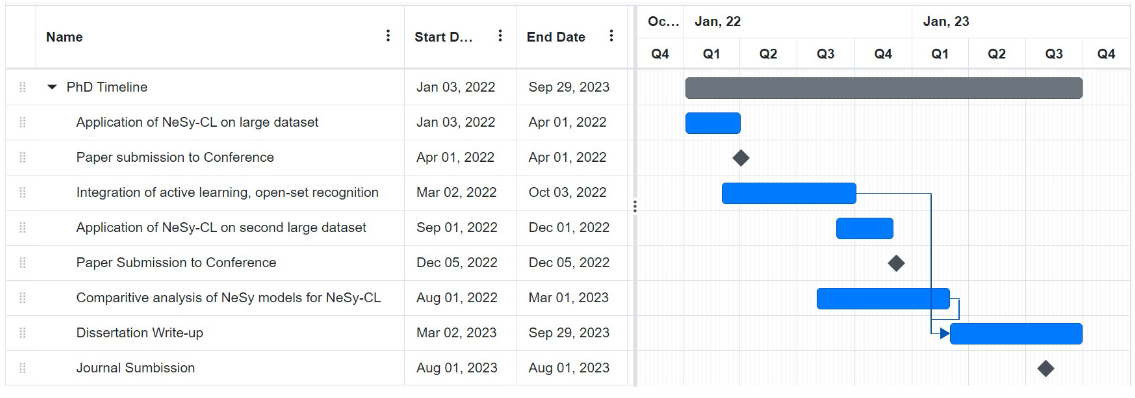
\includegraphics[width=\textwidth]{Images/gantt_chart.png}
\caption{Research timetable}
\label{fig:ResearchTimetable}
\end{figure}

%\input{6-Section.tex}

%-----------------------------------------------------------------------------------------------------------

%---------------------------------------------------------------------------------------------------------------

%bibliography
%\bibliographystyle{agsm}%fror odd Harvard

\bibliographystyle{abbrv}
\bibliography{references.bib}

% Commented out from Mirela's original
%\begin{appendices}
%\section{Workshop Plan}

%This is the submitted and accepted workshop plan for the first study. 
%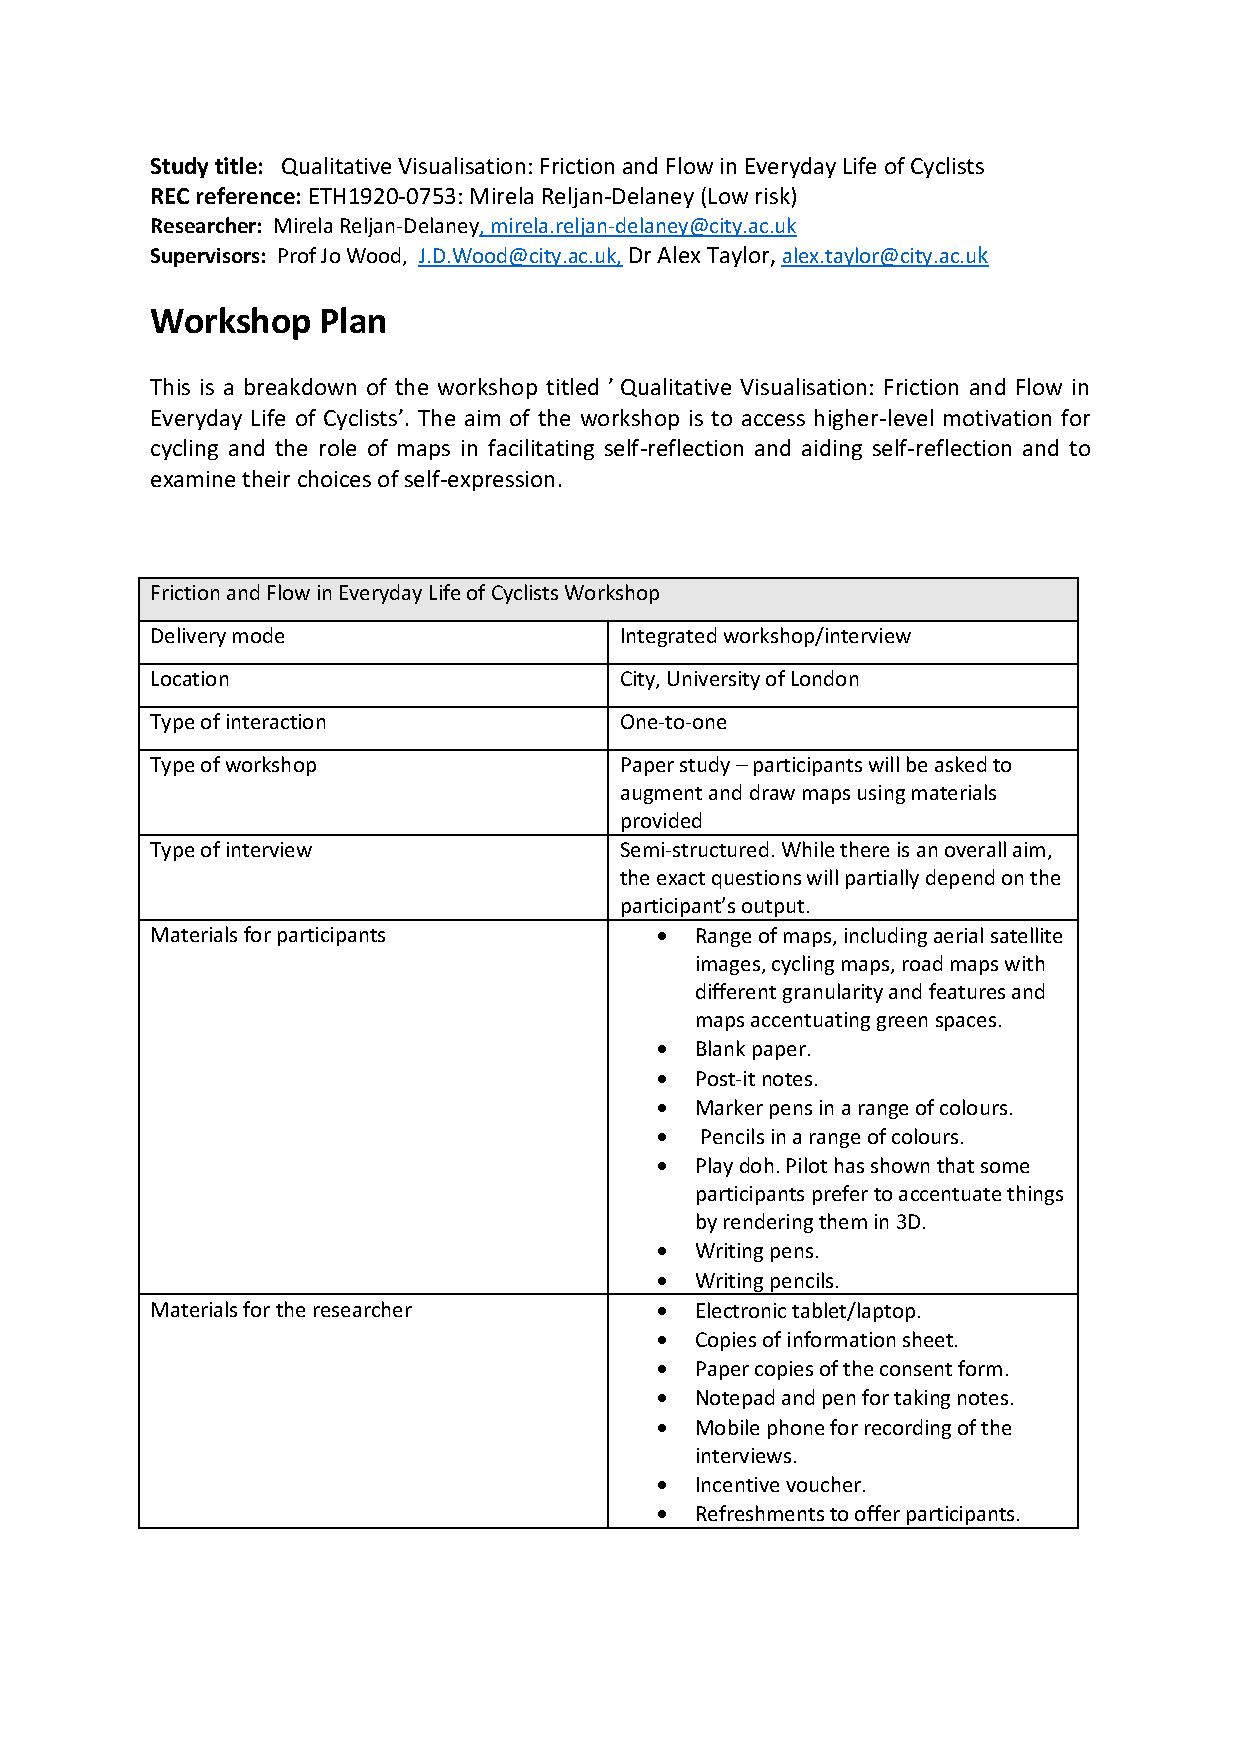
\includegraphics[height=.96\textheight]{Appendix/workshop_plan.pdf}
%\includepdf[pages=2-4]{Appendix/workshop_plan.pdf}
%\label{Appendix 1}

%\section{Example of transcribed and coded interview}


%This is the submitted and accepted workshop plan for the first study. 
%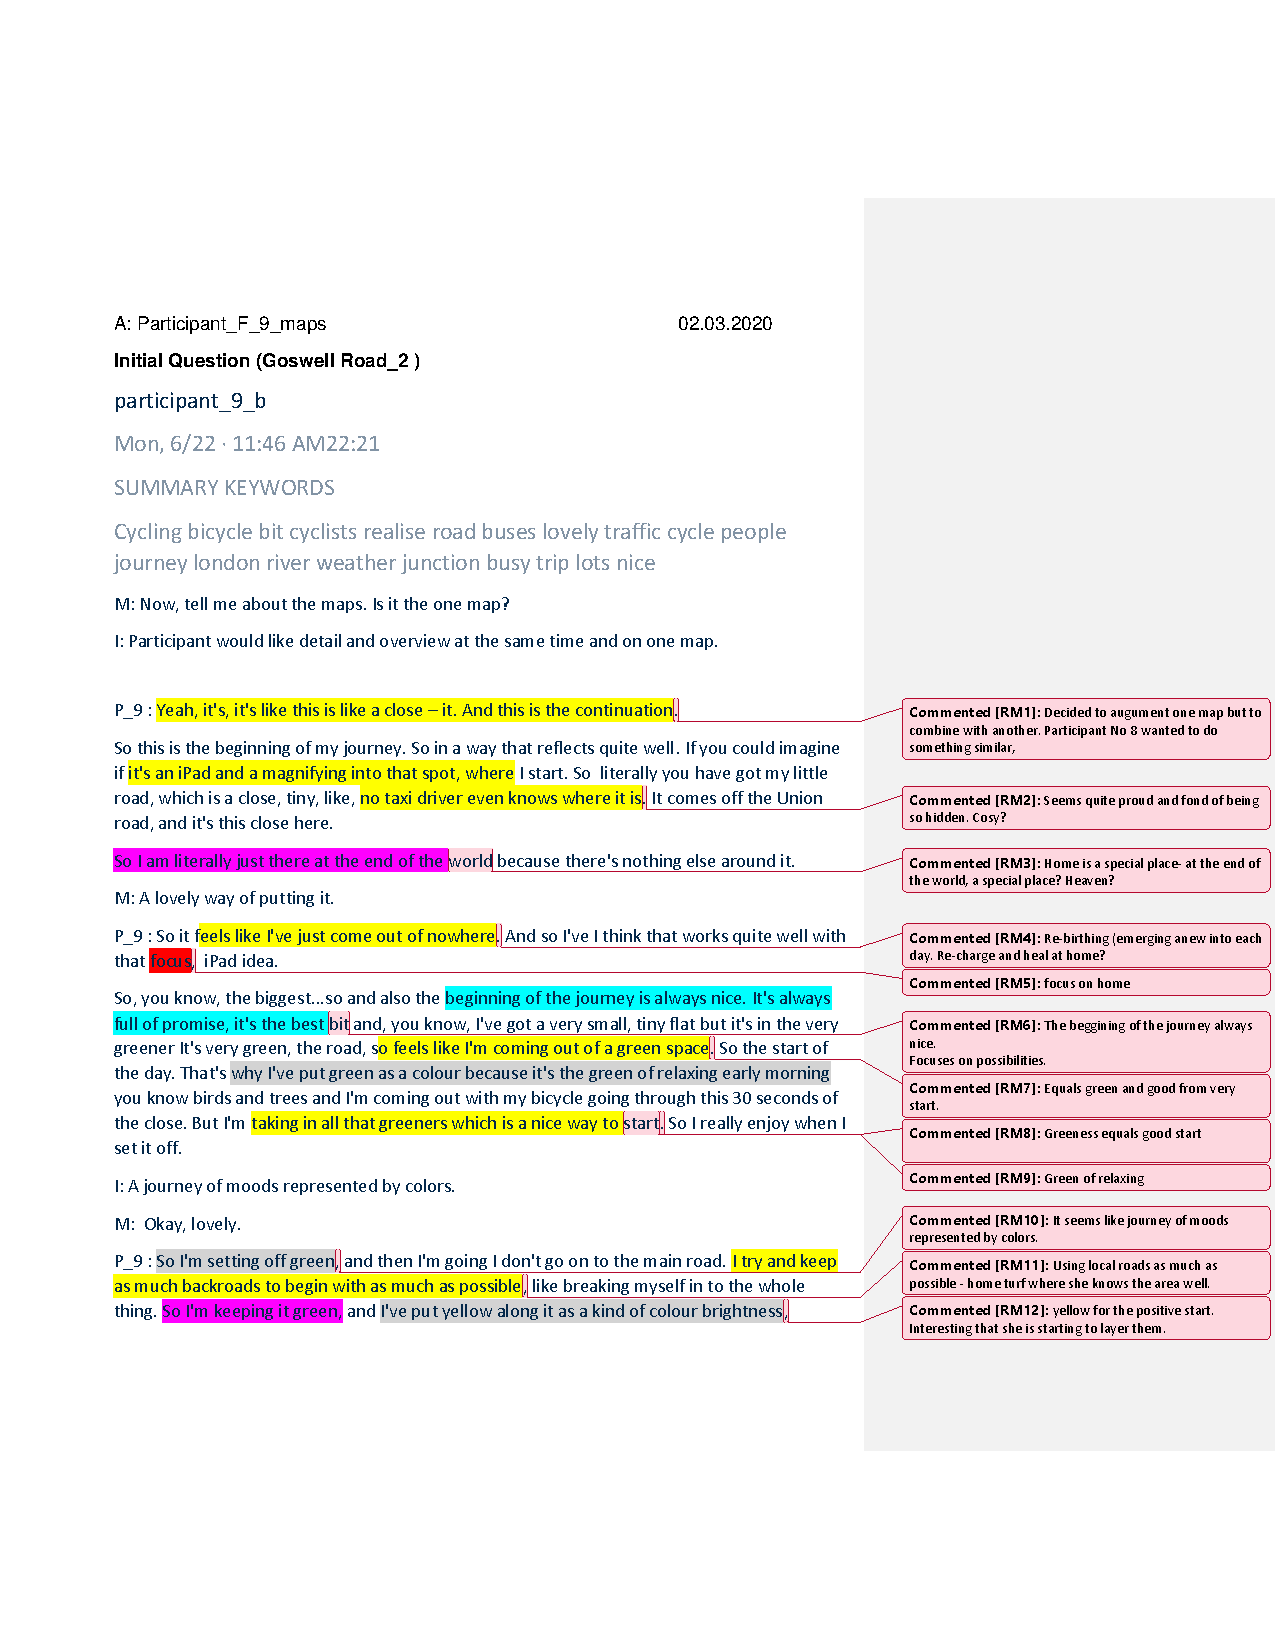
\includegraphics[height=.80\textheight]{Appendix/participant_9-maps.pdf}
%\includepdf[pages=2-5]{Appendix/participant_9-maps.pdf}
%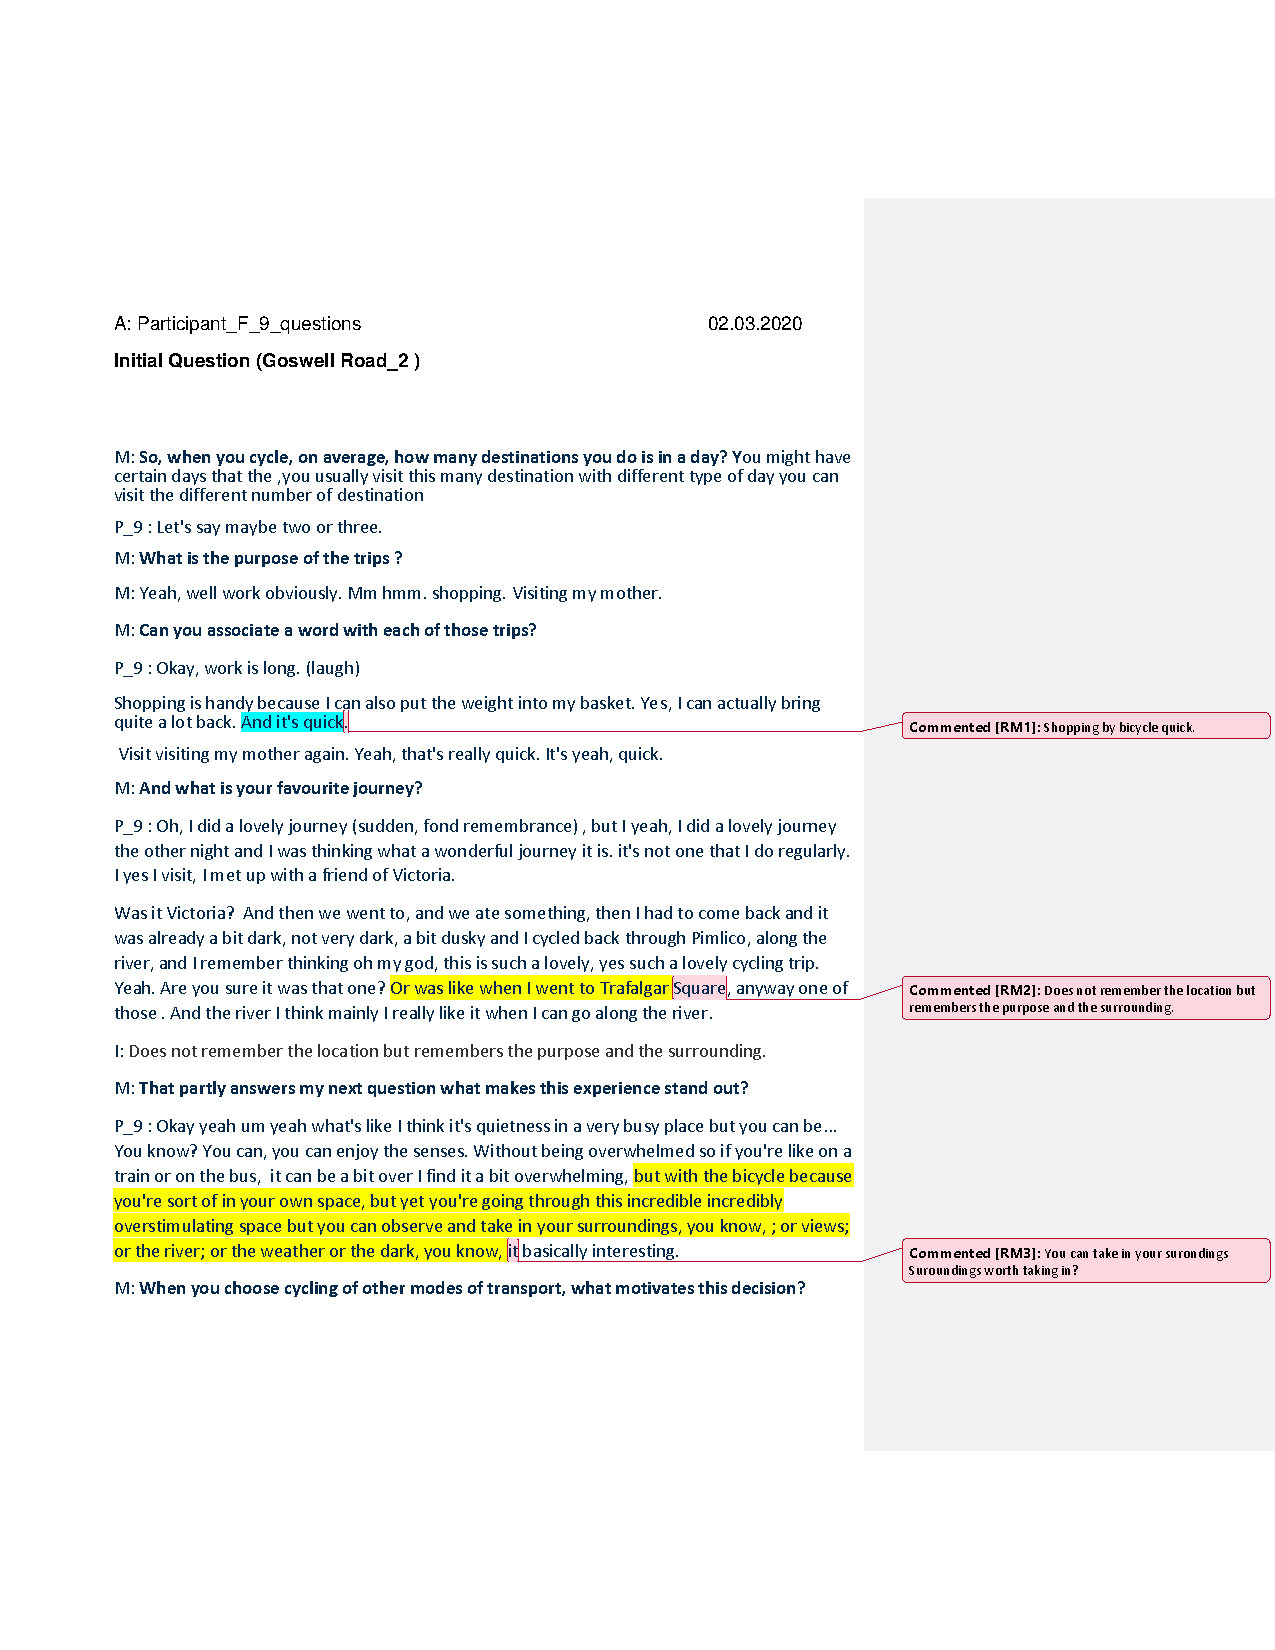
\includepdf[pages=1-3]{Appendix/participant_9-questions.pdf}
%\label{Appendix 2}
%\end{appendices}

\end{document}